% Project structure
%!TEX root = ../Project.tex
\section{Project Structure and Specification}

\begin{figure}[htbp]
	\centering
		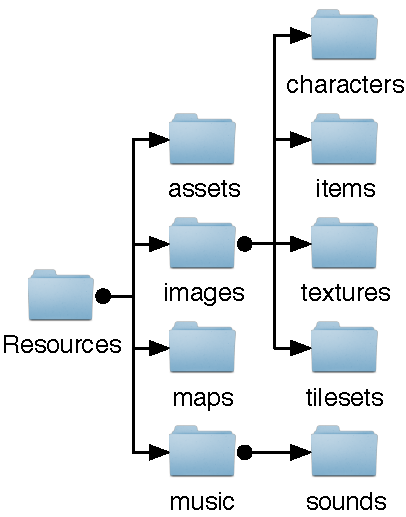
\includegraphics[height=3in]{figures/Files.pdf}
	\caption{Project Structure}
	\label{fig:figures_Files}
\end{figure}

A game's resources  are organised as shown above. The one of the main restistions, is that all to external links have to relative to \texttt{resources} directory. All \texttt{xml} files must conform in the schemas in the \texttt{schemas} directory. 

\subsection{Assets}
Assets are store in following format:
\begin{lstlisting}[caption=Assets format]
<name>
  <entry>
    <uuid>128bit</uuid>
    <resource uuid="128 bit">
    </resource>
  </entry>
</name>
\end{lstlisting}

and \textbf{must} contain the following files conforming to schemas in \texttt{schemas/assets}.
\begin{lstlisting}[caption=Required Assets]
maps.xml
music.xml
ordering.xml
skills.xml
sounds.xml
textures.xml
tilesets.xml
units.xml
unitsImages.xml
weapons.xml
\end{lstlisting}

\subsection{images}
All images are stored as sprite sheets(see section \ref{ssub:sprite_sheets}).  There \emph{three} required files for each sprite sheet. 
\begin{lstlisting}
name.png
name.xml
name-animations.xml
\end{lstlisting}
The sprite sheet itself is stored in a Portable Network Graphics(png) format which is contained in \texttt{name.png}. \texttt{name.xml} contains the cordaties of the images in the sprite sheet as well as the size of the sheet. \texttt{name-animations.xml} contains the unique id of the sprite sheet and can optional specify animations. 

\subsection{Maps}
\label{sub:amaps}

Each map needs the following \emph{five} files:
\begin{description}
	\item[name.xml] which contains the tile information as well references to the other files. 
	\item[name-conditions.xml]  which include among others infomation the  winning conditions. 
	\item[default-enemies.xml]  which contains the enemies data along with their positions on the map.
	\item[default-events.xml]   which contains the dialog at the start and end of battle if any.
	\item[default-music.xml]    which contains the background music and sound effect.
\end{description}

Maps also need a \texttt{tilemaping} which maps the tile types to their images.  A default mapping is created by the editor when a tileset is saved with the name \texttt{tileset-mapping.xml}.

\subsection{Music}
The engine supports only Ogg Vorbis which is ``a completely open, patent-free, professional audio encoding and streaming technology''.
%TODO ref http://www.vorbis.com/
Compared with other format such as MP3, Ogg Vorbis has no lieancely issues. 

\subsection{Sound Effects}
Sound effect can either be Ogg Vorbis, or wave(.wav) format. 

\clearpage
\subsection{Editor}
For the editor the follow structure is used.

\begin{figure}[htbp]
	\centering
		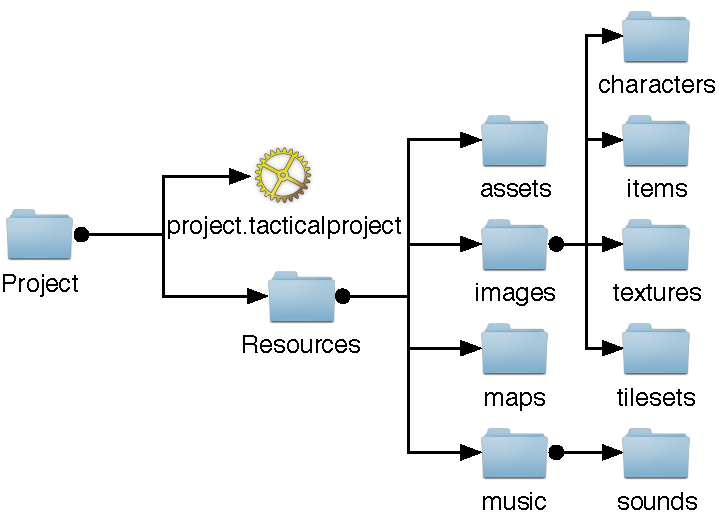
\includegraphics[height=3in]{figures/project.pdf}
	\caption{Editor Project Structure}
	\label{fig:figures_project}
\end{figure}

The main change is the addition of \texttt{project.tacticalproject} file which contains settings specify to the editor. It also has the added benefit allows the user to click on the \texttt{project.tacticalproject} to open the editor if using the Mac version.